%%%%%%%%%%%%%%%%%%%%%%%%%%%%%%%%%%%%%%%%%%%%%%%%%%%%%%%%%%%%%%%%%%%%%%%%%%%%%%%%
% TUM-Vorlage: Präsentation
%%%%%%%%%%%%%%%%%%%%%%%%%%%%%%%%%%%%%%%%%%%%%%%%%%%%%%%%%%%%%%%%%%%%%%%%%%%%%%%%
%
% Rechteinhaber:
%     Technische Universität München
%     https://www.tum.de
% 
% Gestaltung:
%     ediundsepp Gestaltungsgesellschaft, München
%     http://www.ediundsepp.de
% 
% Technische Umsetzung:
%     eWorks GmbH, Frankfurt am Main
%     http://www.eworks.de
%
%%%%%%%%%%%%%%%%%%%%%%%%%%%%%%%%%%%%%%%%%%%%%%%%%%%%%%%%%%%%%%%%%%%%%%%%%%%%%%%%


%%%%%%%%%%%%%%%%%%%%%%%%%%%%%%%%%%%%%%%%%%%%%%%%%%%%%%%%%%%%%%%%%%%%%%%%%%%%%%%%
% Zur Wahl des Seitenverhältnisses bitte einen der beiden folgenden Befehle
% auskommentieren und den ausführen lassen:
\documentclass[t]{beamer}
\usepackage[
    orientation=landscape,
    size=custom,
    width=25.4,
    height=19.05,
    scale=0.63 % erzeugt 16pt Schriftgröße
]{beamerposter}

\newcommand{\PraesentationSchriftgroesseSehrGross}{\fontsize{30}{45}}
\newcommand{\PraesentationSchriftgroesseGross}{\fontsize{22}{33}}
\newcommand{\PraesentationSchriftgroesseNormal}{\fontsize{16}{29}}
\newcommand{\PraesentationSchriftgroesseKlein}{\fontsize{12}{18}}
\newcommand{\PraesentationSchriftgroesseDreizeiler}{\fontsize{7}{10}}
\newcommand{\PraesentationSchriftgroesseAufzaehlungszeichen}{\fontsize{10}{8}}

\newcommand{\PraesentationAbstandAbsatz}{22.1pt}
\newcommand{\PraesentationPositionKorrekturOben}{0cm}
\newcommand{\PraesentationBeispieleSchriftgroessen}{30 | 22 | 16 | 12}
\documentclass[10pt]{scrlttr2} % Dokumentenklasse: KOMA-Skript Letter

% Anpassbare Kopf- und Fußzeilen für KOMA-Skript:
%\usepackage{scrlayer-scrpage}

\usepackage[utf8]{inputenc} % Textkodierung: UTF-8
\usepackage[T1]{fontenc} % Zeichensatzkodierung

\usepackage{calc} % Berechnungen

\usepackage[ngerman]{babel} % Deutsche Lokalisierung
\usepackage{graphicx} % Grafiken
\usepackage[absolute]{textpos} % Positionierung

% Silbentrennung:
\usepackage{hyphenat}
%\tolerance 2414
%\hbadness 2414
%\emergencystretch 1.5em
%\hfuzz 0.3pt
%\widowpenalty=10000     % Hurenkinder
%\clubpenalty=10000      % Schusterjungen
%\vfuzz \hfuzz

% Euro-Symbol:
\usepackage[gen]{eurosym}
\DeclareUnicodeCharacter{20AC}{\euro{}}

% Schriftart Helvetica:
\usepackage[scaled]{helvet}
\renewcommand{\familydefault}{\sfdefault}

\usepackage{mathptmx} % skalierbare Formelschriften
\usepackage{xstring} % Textmanipulation
\usepackage{xcolor} % Farbdefinitionen

\usepackage{etoolbox} % Toggle-Definitionen
\newtoggle{StellenausschreibungGrafikOpportunities}
\togglefalse{StellenausschreibungGrafikOpportunities}

% Debugging:
%\usepackage{layout} % Layout-Informationen
%\usepackage{printlen} % Längenwerte ausgeben
 % Seitenverhältnis 4:3
% %\documentclass[aspectratio=169]{beamer}
\documentclass[t,aspectratio=169]{beamer}
\usepackage[
    orientation=landscape,
    size=custom,
    width=25.4,
    height=14.2875,
    scale=0.5
]{beamerposter}

\newcommand{\PraesentationSchriftgroesseSehrGross}{\fontsize{25}{38}}
\newcommand{\PraesentationSchriftgroesseGross}{\fontsize{18}{27}}
\newcommand{\PraesentationSchriftgroesseNormal}{\fontsize{14}{21}}
\newcommand{\PraesentationSchriftgroesseKlein}{\fontsize{11}{17}}
\newcommand{\PraesentationSchriftgroesseDreizeiler}{\fontsize{7}{10}}
\newcommand{\PraesentationSchriftgroesseAufzaehlungszeichen}{\fontsize{10}{8}}

\newcommand{\PraesentationAbstandAbsatz}{18pt}
\newcommand{\PraesentationPositionKorrekturOben}{-1cm}
\newcommand{\PraesentationBeispieleSchriftgroessen}{25 | 18 | 14 | 11}
\documentclass[10pt]{scrlttr2} % Dokumentenklasse: KOMA-Skript Letter

% Anpassbare Kopf- und Fußzeilen für KOMA-Skript:
%\usepackage{scrlayer-scrpage}

\usepackage[utf8]{inputenc} % Textkodierung: UTF-8
\usepackage[T1]{fontenc} % Zeichensatzkodierung

\usepackage{calc} % Berechnungen

\usepackage[ngerman]{babel} % Deutsche Lokalisierung
\usepackage{graphicx} % Grafiken
\usepackage[absolute]{textpos} % Positionierung

% Silbentrennung:
\usepackage{hyphenat}
%\tolerance 2414
%\hbadness 2414
%\emergencystretch 1.5em
%\hfuzz 0.3pt
%\widowpenalty=10000     % Hurenkinder
%\clubpenalty=10000      % Schusterjungen
%\vfuzz \hfuzz

% Euro-Symbol:
\usepackage[gen]{eurosym}
\DeclareUnicodeCharacter{20AC}{\euro{}}

% Schriftart Helvetica:
\usepackage[scaled]{helvet}
\renewcommand{\familydefault}{\sfdefault}

\usepackage{mathptmx} % skalierbare Formelschriften
\usepackage{xstring} % Textmanipulation
\usepackage{xcolor} % Farbdefinitionen

\usepackage{etoolbox} % Toggle-Definitionen
\newtoggle{StellenausschreibungGrafikOpportunities}
\togglefalse{StellenausschreibungGrafikOpportunities}

% Debugging:
%\usepackage{layout} % Layout-Informationen
%\usepackage{printlen} % Längenwerte ausgeben
 % Seitenverhältnis 16:9
%%%%%%%%%%%%%%%%%%%%%%%%%%%%%%%%%%%%%%%%%%%%%%%%%%%%%%%%%%%%%%%%%%%%%%%%%%%%%%%%


%%%%%%%%%%%%%%%%%%%%%%%%%%%%%%%%%%%%%%%%%%%%%%%%%%%%%%%%%%%%%%%%%%%%%%%%%%%%%%%%
%%%%%%%%%%%%%%%%%%%%%%%%%%%%%%%%%%%%%%%%%%%%%%%%%%%%%%%%%%%%%%%%%%%%%%%%%%%%%%%%
% TUM-Vorlage: Personenspezifische Informationen
%%%%%%%%%%%%%%%%%%%%%%%%%%%%%%%%%%%%%%%%%%%%%%%%%%%%%%%%%%%%%%%%%%%%%%%%%%%%%%%%
%
% Rechteinhaber:
%     Technische Universität München
%     https://www.tum.de
% 
% Gestaltung:
%     ediundsepp Gestaltungsgesellschaft, München
%     http://www.ediundsepp.de
% 
% Technische Umsetzung:
%     eWorks GmbH, Frankfurt am Main
%     http://www.eworks.de
%
%%%%%%%%%%%%%%%%%%%%%%%%%%%%%%%%%%%%%%%%%%%%%%%%%%%%%%%%%%%%%%%%%%%%%%%%%%%%%%%%

% Für die Person anpassen:

\newcommand{\PersonTitel}{Dr.~rer.~nat.}
\newcommand{\PersonVorname}{Erika}
\newcommand{\PersonNachname}{Mustermann}
\newcommand{\PersonStadt}{@Ort@}
\newcommand{\PersonAdresse}{%
    @Adresse@\\%
    @Plz@~\PersonStadt%
}
\newcommand{\PersonTelefon}{@Telefon@}
\newcommand{\PersonFax}{@Fax@}
\newcommand{\PersonEmail}{@E-Mail@}
\newcommand{\PersonWebseite}{@Web@}

\newcommand{\FakultaetAnsprechpartner}{@Ansprechpartner@}
% Fakultät:
\newcommand{\FakultaetName}{@Fakultät@}
\newcommand{\LehrstuhlName}{@Lehrstuhlname@}

\newcommand{\EinstellungBankName}{Bayerische Landesbank}
\newcommand{\EinstellungBankIBAN}{DE10700500000000024866}
\newcommand{\EinstellungBankBIC}{BYLADEMM}
\newcommand{\EinstellungSteuernummer}{143/241/80037}
\newcommand{\EinstellungUmsatzsteuerIdentifikationsnummer}{DE811193231}

\hyphenation{} % eigene Silbentrennung                    % !!! DATEI ANPASSEN !!!
%%%%%%%%%%%%%%%%%%%%%%%%%%%%%%%%%%%%%%%%%%%%%%%%%%%%%%%%%%%%%%%%%%%%%%%%%%%%%%%%


\renewcommand{\PersonTitel}{Dr. rer. nat.}
\newcommand{\Datum}{\today}

\renewcommand{\PraesentationFusszeileZusatz}{| kann beliebig erweitert werden | Infos mit Strich trennen}

\title{Titel der Präsentation bearbeiten}
\author{\PersonTitel{} \PersonVorname{} \PersonNachname}
\institute[]{\UniversitaetName \\ \FakultaetName \\ \LehrstuhlName}
\date[\Datum]{München, 27. März 2015}
\subject{Thema der Präsentation}


%%%%%%%%%%%%%%%%%%%%%%%%%%%%%%%%%%%%%%%%%%%%%%%%%%%%%%%%%%%%%%%%%%%%%%%%%%%%%%%%
%%%%%%%%%%%%%%%%%%%%%%%%%%%%%%%%%%%%%%%%%%%%%%%%%%%%%%%%%%%%%%%%%%%%%%%%%%%%%%%%
% EINSTELLUNGEN
%%%%%%%%%%%%%%%%%%%%%%%%%%%%%%%%%%%%%%%%%%%%%%%%%%%%%%%%%%%%%%%%%%%%%%%%%%%%%%%%

% Allgemein:
\newcommand{\AllgemeinGestalter}{ediundsepp Gestaltungsgesellschaft}
\newcommand{\AllgemeinErsteller}{eWorks GmbH}

% Universität:
\newcommand{\UniversitaetName}{Technische Universität München}
\newcommand{\UniversitaetAbkuerzung}{TUM}
\newcommand{\UniversitaetWebseite}{www.tum.de}
\newcommand{\UniversitaetLogoBreite}{19mm}
\newcommand{\UniversitaetLogoHoehe}{1cm}

\newcommand{\UniversitaetAdresse}{%
    Arcisstraße~21\\%
    80333~München%
}


% Seitenränder:
\newcommand{\SeitenrandOben}{20mm}
\newcommand{\SeitenrandRechts}{20mm}
\newcommand{\SeitenrandLinks}{25mm}
\newcommand{\SeitenrandUnten}{10mm}

% Falzmarken:
\newcommand{\FalzmarkeOben}{87mm}
\newcommand{\FalzmarkeMitte}{148.5mm}
\newcommand{\FalzmarkeUnten}{192mm}
\newcommand{\FalzmarkeBreite}{2mm}
\newcommand{\FalzmarkeDicke}{0.3pt}
\newcommand{\FalzmarkePositionLinks}{7mm}


% Adressfeld:
\newcommand{\AdressfeldHoehe}{45mm}
\newcommand{\AdressfeldBreite}{85mm}
\newcommand{\AdressfeldAbsenderSchriftgroesse}{7.5pt}
\newcommand{\AdressfeldEmpfaengerSchriftgroesse}{11pt}
\newcommand{\AdressfeldEmpfaengerZeilenabstand}{15pt}

% Text:
\newcommand{\TextOben}{77.5mm}
\newcommand{\TextSchriftgroesse}{11pt}
\newcommand{\TextZeilenabstand}{15pt}

% Fusszeile:
\newcommand{\FusszeilePositionOben}{271mm}
\newcommand{\FusszeileBreite}{165mm}
\newcommand{\FusszeileHoehe}{16.5mm}
\newcommand{\FusszeileZwischenabstand}{2mm}
\newcommand{\FusszeileBreiteGross}{44mm}
\newcommand{\FusszeileBreiteKlein}{35.5mm}
\newcommand{\FusszeileSeitennummerAbstand}{7.7mm}
\newcommand{\FusszeileSchriftgroesse}{7.5pt}
\newcommand{\FusszeileZeilenabstand}{8pt}


%%%%%%%%%%%%%%%%%%%%%%%%%%%%%%%%%%%%%%%%%%%%%%%%%%%%%%%%%%%%%%%%%%%%%%%%%%%%%%%%
% DOKUMENT
%%%%%%%%%%%%%%%%%%%%%%%%%%%%%%%%%%%%%%%%%%%%%%%%%%%%%%%%%%%%%%%%%%%%%%%%%%%%%%%%

\usepackage[a4paper,
    top=\SeitenrandOben,
    bottom=\SeitenrandUnten,
    inner=\SeitenrandLinks,
    outer=\SeitenrandRechts,
    foot=\FusszeileHoehe - 1mm,
    head=0cm,
    includefoot
]{geometry}

\textblockorigin{\SeitenrandLinks}{\SeitenrandOben} % Ursprung für Positionierung

% PDF-Einstellungen:
\usepackage[pdftex]{hyperref}
\hypersetup{
    hidelinks,
    pdfauthor={\PersonVorname{} \PersonNachname},
    pdftitle={\Betreff},
    pdfproducer={\AllgemeinErsteller},
    pdfcreator={\AllgemeinGestalter}
}

\renewcommand*{\raggedsignature}{\raggedright}

\makeatletter
    \@setplength{bfoldmarklength}{\FalzmarkeBreite}
    \@setplength{bfoldmarkvpos}{\FalzmarkeUnten}
    \@setplength{firstfoothpos}{\SeitenrandLinks - 2pt}
    \@setplength{firstfootvpos}{\FusszeilePositionOben}
    \@setplength{firstfootwidth}{\FusszeileBreite}
    \@setplength{foldmarkhpos}{\FalzmarkePositionLinks}
    \@setplength{foldmarkthickness}{\FalzmarkeDicke}
    \@setplength{mfoldmarklength}{\FalzmarkeBreite}
    \@setplength{mfoldmarkvpos}{\FalzmarkeMitte}

    \@setplength{refaftervskip}{\TextZeilenabstand}
    \@setplength{refvpos}{\TextOben}
    \@setplength{sigbeforevskip}{\baselineskip}
    \@setplength{sigindent}{0mm}
    \@setplength{subjectaftervskip}{\baselineskip + \baselineskip + 1pt}

    \@setplength{tfoldmarklength}{\FalzmarkeBreite}
    \@setplength{tfoldmarkvpos}{\FalzmarkeOben}
\makeatother

\KOMAoptions{
    fontsize=\TextSchriftgroesse,
    foldmarks=BMpTv,
    firsthead=false,
    backaddress=no,
    addrfield=no,
    fromalign=false
}

\setkomavar{fromname}{\UniversitaetName}
\setkomavar{fromaddress}{\PersonAdresse}
\addtokomafont{backaddress}{\fontsize{\AdressfeldAbsenderSchriftgroesse}{\AdressfeldAbsenderSchriftgroesse}\selectfont}
\addtokomafont{toaddress}{\fontsize{\AdressfeldEmpfaengerSchriftgroesse}{\AdressfeldEmpfaengerZeilenabstand}\selectfont}

\newcommand{\RuecksendeadresseTrenner}{~| \ignorespaces}

\AtBeginLetter{%
    % Logo:
    \begin{textblock*}{\UniversitaetLogoBreite}[1,0](\textwidth, 0cm)%
        \raggedleft%
        
\includegraphics{./Ressourcen/_Bilder/Universitaet_Logo_RGB.pdf}%
    \end{textblock*}%
    \setlength{\baselineskip}{\TextZeilenabstand}%
    \setlength{\parindent}{0mm} % keine Einrückung am Absatzanfang
    \setlength{\parskip}{\baselineskip} % einzeiliger Abstand nach Absätzen
    % Empfängerfenster:
    \begin{textblock*}{\AdressfeldBreite}[0,0](0cm, 15mm)%
        \raggedbottom\raggedright
        \begin{spacing}{.85}%
        {
            \usekomafont{backaddress}%
            \let\\\RuecksendeadresseTrenner% Umdefinieren von "\\" zu "~| "
            \Absender%
        } \\
        \end{spacing}
        \vspace*{5.5pt}
        \usekomafont{toaddress}%
        \EmpfaengerAdresse
    \end{textblock*}
}

\KOMAoptions{refline=dateleft}
\setkomavar{date}{\Datum}
\setkomavar{place}{\PersonStadt}
\setkomafont{subject}{\bfseries}
\setkomavar{subject}{\Betreff}
\setkomavar{signature}{\PersonVorname~\PersonNachname}

%\setkomavar*{enclseparator}{Anlage\vspace{-3em}}

\renewcommand*{\closing}[1]{#1\vspace*{3\baselineskip}\newline\usekomavar{signature}\newline}
\setkomavar{enclseparator}[Anlage]{~}
\renewcommand{\encl}[1]{\newline{}Anlage~#1}

\KOMAoptions{firstfoot=true}
\setkomafont{pagefoot}{\sffamily\fontsize{7.5pt}{8pt}\selectfont}
\renewcommand{\pagemark}{%
\begin{textblock*}{3em}[1,1](\paperwidth - \SeitenrandLinks - \SeitenrandRechts + \FusszeileSeitennummerAbstand + 3mm, \paperheight - \SeitenrandOben - \SeitenrandUnten)%
    \raggedleft\hfill\usekomafont{pagefoot}\thepage\,/\,\pageref*{LastPage}%
\end{textblock*}%
}

\setkomavar{firstfoot}{
    \TabPositions{2em}%
    \begin{minipage}[t][\FusszeileHoehe][t]{\FusszeileBreiteGross}%
        \usekomafont{pagefoot}%
        \textbf{\UniversitaetName}%
        \newline%
        \FakultaetName%
        \newline%
        \LehrstuhlName%
    \end{minipage}%
    \hspace*{\FusszeileZwischenabstand}%
    \begin{minipage}[t][\FusszeileHoehe][t]{\FusszeileBreiteGross}%
        \raggedright\usekomafont{pagefoot}%
        \textbf{\FakultaetAnsprechpartner}\newline%
        \PersonAdresse%
    \end{minipage}%
    \hspace*{\FusszeileZwischenabstand}%
    \begin{minipage}[t][\FusszeileHoehe][t]{\FusszeileBreiteKlein}%
        \raggedright\usekomafont{pagefoot}%
        Tel.\tab{\PersonTelefon}%
        \def\temp{\PersonFax}\ifx\temp\empty%
        \else%
          \newline Fax\tab{\PersonFax}%
        \fi%
        \newline\newline%
        \PersonEmail\newline%
        \href{http://\PersonWebseite}{\PersonWebseite}\newline%
        \href{http://\UniversitaetWebseite}{\UniversitaetWebseite}%
    \end{minipage}%
    \hspace*{\FusszeileZwischenabstand}%
    \begin{minipage}[t][\FusszeileHoehe][t]{\FusszeileBreiteKlein}%
        \raggedright\usekomafont{pagefoot}%
        \EinstellungBankName\newline%
        IBAN-Nr.: \EinstellungBankIBAN\newline%
        BIC: \EinstellungBankBIC\newline%
        Steuer-Nr.: \EinstellungSteuernummer\newline%
        USt-IdNr.: \EinstellungUmsatzsteuerIdentifikationsnummer\newline%
    \end{minipage}%
    \pagemark%
}

\begin{document}
\raggedright
\begin{letter}{\EmpfaengerAdresse{}}
\opening{\Gruss}

 % !!! NICHT ENTFERNEN !!!
%%%%%%%%%%%%%%%%%%%%%%%%%%%%%%%%%%%%%%%%%%%%%%%%%%%%%%%%%%%%%%%%%%%%%%%%%%%%%%%%


%%%%%%%%%%%%%%%%%%%%%%%%%%%%%%%%%%%%%%%%%%%%%%%%%%%%%%%%%%%%%%%%%%%%%%%%%%%%%%%%
% FOLIENSTIL: Standard
% !!!ÄNDERUNG HIER:!!!
\PraesentationMasterStandard

\PraesentationTitelseite % Fügt die Startseite ein


%%%%%%%%%%%%%%%%%%%%%%%%%%%%%%%%%%%%%%%%%%%%%%%%%%%%%
%% Beispielfolien                                  %%
%%%%%%%%%%%%%%%%%%%%%%%%%%%%%%%%%%%%%%%%%%%%%%%%%%%%%%%%%%%%%%%%%%%%%%%%%%%%%%%%
% TUM-Vorlage: Präsentation - Beispiele
%%%%%%%%%%%%%%%%%%%%%%%%%%%%%%%%%%%%%%%%%%%%%%%%%%%%%%%%%%%%%%%%%%%%%%%%%%%%%%%%


%%%%%%%%%%%%%%%%%%%%%%%%%%%%%%%%%%%%%%%%%%%%%%%%%%%%%
%% Folie: Gültigkeit der Masterfolien              %%
%%%%%%%%%%%%%%%%%%%%%%%%%%%%%%%%%%%%%%%%%%%%%%%%%%%%%

\begin{frame}
    \frametitle{Gültigkeit der Masterfolien}

Dieser Folienmaster gilt bei offiziellen Präsentationen im Rahmen der TUM. Es
ist darauf zu achten, dass wir uns in einem durchgängigen Layout präsentieren.

Abweichungen vom vorgegebenen Layout bitte auf ein Minimum reduzieren.

\end{frame}
\clearpage


%%%%%%%%%%%%%%%%%%%%%%%%%%%%%%%%%%%%%%%%%%%%%%%%%%%%%
%% Folie: Grundlage der Masterfolien               %%
%%%%%%%%%%%%%%%%%%%%%%%%%%%%%%%%%%%%%%%%%%%%%%%%%%%%%

\begin{frame}
    \frametitle{Grundlage der Masterfolien}

Als Grundlage dient der Corporate Design Style Guide der TUM.\newline
Die Präsentationsvorlage ist auf gute Lesbarkeit und klare Darstellung von
Informationen optimiert.

\end{frame}
\clearpage


%%%%%%%%%%%%%%%%%%%%%%%%%%%%%%%%%%%%%%%%%%%%%%%%%%%%%
%% Folie: 2-zeilige Überschrift                    %%
%%%%%%%%%%%%%%%%%%%%%%%%%%%%%%%%%%%%%%%%%%%%%%%%%%%%%

\begin{frame}
    \PraesentationUeberschriftZweizeilig{Hier steht eine}{2-zeilige Überschrift}

Als Grundlage dient der Corporate Design Style Guide der TUM.\newline
Die Präsentationsvorlage ist auf gute Lesbarkeit und klare Darstellung von
Informationen optimiert.

\end{frame}
\clearpage


%%%%%%%%%%%%%%%%%%%%
%% Folie: Schrift %%
%%%%%%%%%%%%%%%%%%%%
\begin{frame}
    \frametitle{Schrift}

Das Grundprinzip ist, Informationen bestmöglich zu transportieren. Dazu muss
vor allem die Schrift einheitlich und für alle im Raum lesbar sein.

Schriftart: Helvetica

Schriftgößen: \PraesentationBeispieleSchriftgroessen

Zeilenabstand: 1,15 mm

Die Einstellungen sind für diese Vorlage als Standard eingestellt. Bei
Diagrammen und Tabellen muss die Schriftgröße ggf. angepasst werden. Für
Ausszeichnungen im Fließtext kann auch \textbf{fett} markiert werden. Bei
großer Distanz bzw. kleinem Präsenationsmedium kann der Schriftgrad notfalls
proportional erhöht werden.

\end{frame}
\clearpage


%%%%%%%%%%%%%%%%%%%
%% Folie: Farben %%
%%%%%%%%%%%%%%%%%%%
\begin{frame}
    \frametitle{Farben}
    
Als erstes soll mit schwarz und weiß gearbeitet werden.\newline
Für Aufwändigere Darstellungen sind Farben mit Bedacht und in möglichst
geringem Umfang einzusetzen.

In diesem Folienmaster ist die Farbpalette festgelegt.

{
    \renewcommand{\arraystretch}{1.2} % skaliert die Tabellen mit Farbfeldern

    Zuerst mit den Primärfarben arbeiten.

    \setlength{\fboxsep}{-1pt} \setlength{\fboxrule}{1pt} % fbox/framebox konfigurieren

    \vspace*{-5mm}
    \begin{tabularx}{\textwidth}{@{} l @{\hspace{4mm}} l @{\hspace{4mm}} l}
        \crule[TUMBlau]{24mm}{6mm}
        & \crule[black]{24mm}{6mm}
        & \fbox{\crule[white]{24mm}{6mm}}
    \end{tabularx}

    \vspace*{-5mm}
    Für z.B. komplexe Diagramme stehen noch Sekundärfarben zur Verfügung.

    \vspace*{-5mm}
    \begin{tabularx}{\textwidth}{@{} l @{\hspace{4mm}} l @{\hspace{4mm}} l @{\hspace{4mm}} l}
        \crule[TUMBlauDunkel]{24mm}{6mm}
        & \crule[TUMBlauMittel]{24mm}{6mm}
        & \crule[TUMBlauHell]{24mm}{6mm}
        & \crule[TUMGrau]{24mm}{6mm}
    \end{tabularx}

    \vspace*{-5mm}
    Bei weiterer Komplexität oder zusätzlichen Markierungen:

    \vspace*{-5mm}
    \begin{tabularx}{\textwidth}{@{} l @{\hspace{4mm}} l @{\hspace{4mm}} l }
        \crule[TUMOrange]{24mm}{6mm}
        & \crule[TUMGruen]{24mm}{6mm}
        & \crule[TUMElfenbein]{24mm}{6mm}
    \end{tabularx}
}

\end{frame}
\clearpage


%%%%%%%%%%%%%%%%%%
%% Folie: Texte %%
%%%%%%%%%%%%%%%%%%
\begin{frame}
    \frametitle{Texte}
 
Kurze und knappe Texte, Fließtexte linksbündig, kein Blocksatz \\[\baselineskip]

Beispiel:\newline
Tem soluptam, nisi as verum ereprehendam at acculpa quidisq uissit volupta
tusdant utem as etur, odi odis es doluptiae dem nimaion con nossinctenis pora
quam voloria consenimus blabore everfer epeliquo maio etur.

\end{frame}
\clearpage


%%%%%%%%%%%%%%%%%%%%%%%
%% Folie: Aufzählung %%
%%%%%%%%%%%%%%%%%%%%%%%
\begin{frame}
    \frametitle{Aufzählung}
    
Bei kleinen Aufzählungen auf Aufzählungszeichen verzichten und ggf. zusätzliche Leerzeile.\newline
Nur die wesentlichen Punkte nennen und Themen auf verschiedene Seiten splitten.\\
Punkt 1\\
Punkt 2

Wenn Unterpunkte in einer Aufzählung nötig sind ist ein Einrücken mit \PraesentationAufzaehlungEbeneZweiSymbol{} möglich

\begin{PraesentationAufzaehlung}
    \item Unterpunkt 1
        \begin{itemize}
            \item Unterpunkt 1
            \item Unterpunkt 2
        \end{itemize}
\end{PraesentationAufzaehlung}

Bei größeren Listen die Standardeinstellung \PraesentationAufzaehlungEbeneEinsSymbol{} verwenden

\begin{PraesentationAufzaehlung}
    \item Unterpunkt 1
    \item Unterpunkt 2
    \item Unterpunkt 3
\end{PraesentationAufzaehlung}

\end{frame}
\clearpage


%%%%%%%%%%%%%%%%%%%%%%%%%%%%%%%
%% Folie: Bilder - Allgemein %%
%%%%%%%%%%%%%%%%%%%%%%%%%%%%%%%
\begin{frame}
    \frametitle{Bilder -- Allgemein}
    
schlichte Darstellung von Informationen \\[\baselineskip]

reduzierte Farben \\[\baselineskip]

Rahmen und Überlagerungen nach Möglichkeit vermeiden \\[\baselineskip]

    
\end{frame}
\clearpage


%%%%%%%%%%%%%%%%%%%%%%%%%%
%% Folie: Bilder - Zwei %%
%%%%%%%%%%%%%%%%%%%%%%%%%%
\begin{frame}
    \frametitle{Bilder}
    
Bildbeschreibung\newline
oberer Bildrand: Begrenzung durch Text\\[\baselineskip]

\mbox{
\includegraphics[height=.5\paperheight, trim=0cm 14cm 0cm 0cm, clip=true]{../Ressourcen/_Bilder/SternenhimmelHochkant.jpg}}%
\hspace{6.5mm}%
\mbox{
\includegraphics[height=.5\paperheight, trim=0cm 14cm 0cm 0cm, clip=true]{../Ressourcen/_Bilder/SternenhimmelHochkant.jpg}}

\end{frame}
\clearpage


%%%%%%%%%%%%%%%%%%%%%%%%%%%%%%%%%%%%%%%%
%% Folie: Bilder - Zweispaltige Seite %%
%%%%%%%%%%%%%%%%%%%%%%%%%%%%%%%%%%%%%%%%
\begin{frame}
    \frametitle{Bilder}

\begin{multicols}{2}
    \textbf{Überschrift 2}\newline
    Hier steht ein einleitender oder beschreibender Fließtext und nach Wunsch
    eine Aufzählung.

    Punkt 1

    Punkt 2

    Punkt 3

    Punkt 4
    \vfill\columnbreak
    
\includegraphics[width=\columnwidth, height=.7\textheight]{../Ressourcen/_Bilder/SternenhimmelHochkant.jpg}%
\end{multicols}
    
\end{frame}
\clearpage


%%%%%%%%%%%%%%%%%%%%%%%%%%%%%%%
%% Folie: Bilder - Textbreit %%
%%%%%%%%%%%%%%%%%%%%%%%%%%%%%%%
\begin{frame}
    \frametitle{Bilder}

Bildbeschreibung\newline
oberer Bildrand: Begrenzung durch Text\\[\baselineskip]


\includegraphics[width=\textwidth, height=.55\textheight]{../Ressourcen/_Bilder/SternenhimmelQuer.jpg}%

\end{frame}
\clearpage


%%%%%%%%%%%%%%%%%%%%%%%%%%%%%%%%%%%%%%%%%%%%%%%%%%
%% Folie: Bilder - seitenbreit mit Beschreibung %%
%%%%%%%%%%%%%%%%%%%%%%%%%%%%%%%%%%%%%%%%%%%%%%%%%%
\begin{frame}
    \frametitle{Bilder}

    Bildbeschreibung\newline
    oberer Bildrand: Begrenzung durch Text

\vspace*{-3mm}
\begin{minipage}[t][0cm]{\paperwidth}%
\hspace*{-\PraesentationSeitenrand}%

\includegraphics[width=\paperwidth]{../Ressourcen/_Bilder/SternenhimmelQuer.jpg}
\end{minipage}
    
\end{frame}
\clearpage


%%%%%%%%%%%%%%%%%%%%%%%%%%%%%%%%%%%%%%%%%%%%%%%%%%%%%
%% Folie: Nicht Format füllende Bilder %%
%%%%%%%%%%%%%%%%%%%%%%%%%%%%%%%%%%%%%%%%%%%%%%%%%%%%%
\begin{frame}
    \frametitle{Nicht Format füllende Bilder}
    
    Weißer bzw. transparenter Hintergrund\newline
    mit genug Freiraum anordnen


\begin{textblock*}{0.4\paperwidth}[0,1](0cm, \textheight - \PraesentationSeitenrand)%
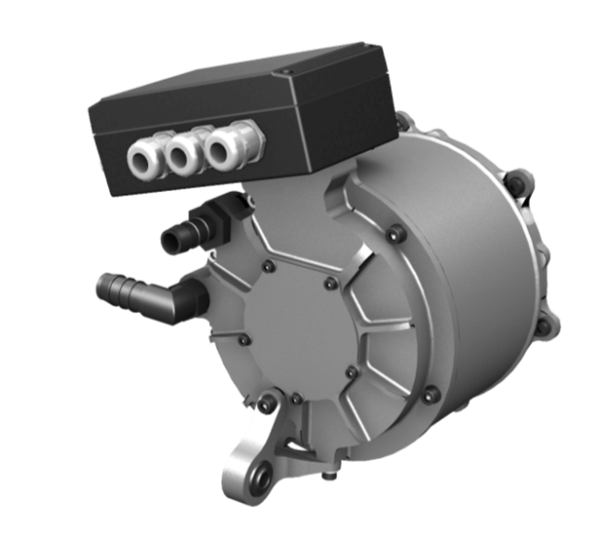
\includegraphics[width=0.4\paperwidth]{../Ressourcen/Praesentation/Bilder/Motor.png}
\end{textblock*}

\begin{textblock*}{0.6\paperwidth}[1,1](\textwidth + \PraesentationSeitenrand, \textheight - \PraesentationSeitenrand)%
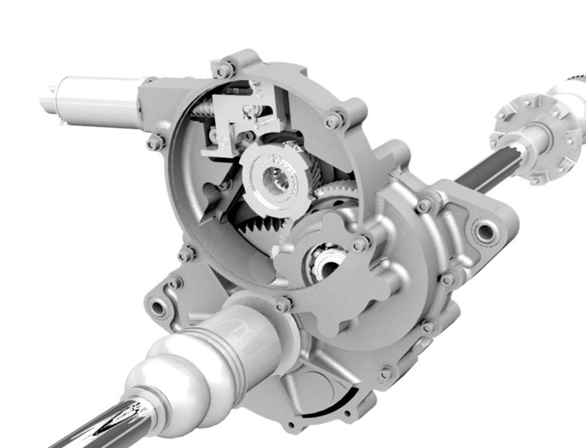
\includegraphics[width=0.6\paperwidth]{../Ressourcen/Praesentation/Bilder/Getriebe.png}
\end{textblock*}

\end{frame}
\clearpage


%%%%%%%%%%%%%%%%%%%%%%%%%%%%%%%%%%%
%% Folie: Bilder - formatfüllend %%
%%%%%%%%%%%%%%%%%%%%%%%%%%%%%%%%%%%
\begin{frame}
    \frametitle{Bilder Format füllend -- maximale Bildgröße}

\begin{minipage}[t][0cm]{\paperwidth}%
\hspace*{-\PraesentationSeitenrand}%

\includegraphics[width=\textwidth]{../Ressourcen/_Bilder/SternenhimmelQuer.jpg}
\end{minipage}
    
\end{frame}
\clearpage


%%%%%%%%%%%%%%%%%%%%%%%%%%%%%%%%%%%%%%%%%%%%%%%%%%%%%
%% Folie: Nicht Format füllende Bilder %%
%%%%%%%%%%%%%%%%%%%%%%%%%%%%%%%%%%%%%%%%%%%%%%%%%%%%%
\begin{frame}
    \frametitle{Nicht Format füllende Bilder}
    
Alternativ mit formatfüllendem Hintergrund: Weiß 5\% dunkler\newline
Beschriftungen können zusätzlich neben den Bildern angebracht werden

\begin{textblock*}{\paperwidth}[0,0](0cm, .4\textheight)%
Bilderklärung
\end{textblock*}

\begin{textblock*}{\paperwidth}[1,0](\textwidth, .4\textheight)%
\raggedleft%
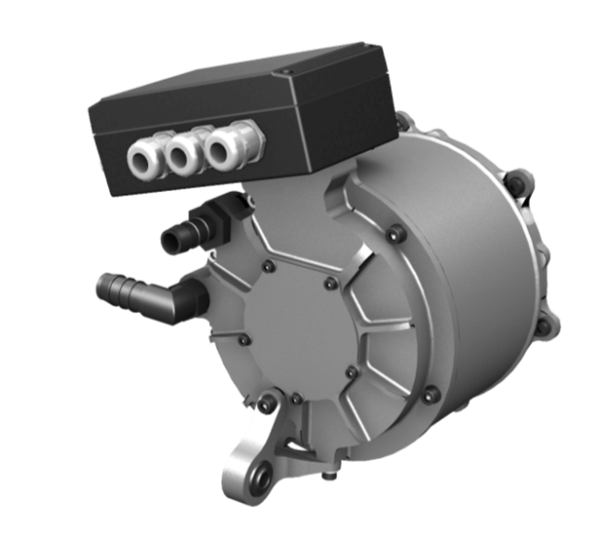
\includegraphics[height=0.5\textheight]{../Ressourcen/Praesentation/Bilder/Motor.png}
\end{textblock*}

\end{frame}
\clearpage


%%%%%%%%%%%%%%%%%%%%%%%%%%%%%%%%%%%%%%%%%%%%%%%%%%%%%
%% Folie: Tabelle - Ohne Rand 					   %%
%%%%%%%%%%%%%%%%%%%%%%%%%%%%%%%%%%%%%%%%%%%%%%%%%%%%%
\begin{frame}
    \frametitle{Tabelle -- Beispiel 1}
    
Tabelle ohne Farbe und kein Rand \\
innerer Seitenrand links 0 cm, um Faktor 1,75 skalierte Tabelle (für genug Zeilenabstand)

\raggedright
{
    \vspace*{0.3pt}
    \renewcommand{\arraystretch}{1.75} % skaliert die Tabelle auf die gewünschte Größe
    \begin{tabularx}{\textwidth}{@{} l @{\hspace{38.7mm}} l}
        Ø - Strecke & 39 km/Tag (14.360 km/Jahr) \\
        Ø - Geschwindigkeit & 25 km/h \\
        Ø - Verfügbare Ladezeit & 22 h/Tag \\
        Kosten   & Kleinwagen mit Verbrennungsmotor \\
        Einsatzgebiet   &  Stadt und Umland
    \end{tabularx}
}
\end{frame}


%%%%%%%%%%%%%%%%%%%%%%%%%%%%%%%%%%%%%%%%%%%%%%%%%%%%%
%% Folie: Tabelle - Mit Rand                       %%
%%%%%%%%%%%%%%%%%%%%%%%%%%%%%%%%%%%%%%%%%%%%%%%%%%%%%
\begin{frame}
    \frametitle{Tabelle -- Beispiel 2}
    
Tabelle ohne Farbe und mit Rand\\
automatische Zelleninnenabstände, um Faktor 1,75 skalierte Tabelle (für genug Zeilenabstand)

\raggedright
{
    \vspace*{0.3pt}
    \renewcommand{\arraystretch}{1.75} % skaliert die Tabelle auf die gewünschte Größe
    \begin{tabularx}{\textwidth}{| l @{\hspace{38.7mm}} | X |}
        \hline
        Ø - Strecke & 39 km/Tag (14.360 km/Jahr) \\ \hline
        Ø - Geschwindigkeit & 25 km/h \\ \hline
        Ø - Verfügbare Ladezeit & 22 h/Tag \\ \hline
        Kosten   & Kleinwagen mit Verbrennungsmotor \\ \hline
        Einsatzgebiet   &  Stadt und Umland \\ \hline
    \end{tabularx}
}
\end{frame}

\clearpage


%%%%%%%%%%%%%%%%%%%%%%%%%%%%%%%%%%%%%%%%%%%%%%%%%%%%%
%% Folie: Diagramme - Beispiel 1                   %%
%%%%%%%%%%%%%%%%%%%%%%%%%%%%%%%%%%%%%%%%%%%%%%%%%%%%%
\begin{frame}
    \frametitle{Diagramme -- Beispiel 1}

Nach Möglichkeit linksbündig bleiben \\
Unnötige Striche und Balken vermeiden

\begin{center}%
    \vspace*{-1cm}
    \begin{tikzpicture}
        \begin{axis}[
                % kein Abstand zwischen Balken:
                xbar=0,
                draw opacity=0,
                bar width=14,
                axis x line=none,
                axis line style={transparent},
                every tick/.style={transparent},
                xmin=0,
                width=\textwidth,
                height=.6\textheight,
                enlarge y limits=0.15,
                symbolic y coords={Kategorie 4,Kategorie 3,Kategorie 2,Kategorie 1},
                ytick=data,
                legend image code/.code={\draw[draw=none] (0cm,-0.12cm) rectangle (0.29cm,0.17cm);}, % Legenden-Symbol  
                legend columns=3,
                reverse legend,
                legend style={
                    fill=none,
                    draw=none,
                    /tikz/every odd column/.append style={column sep=0.07cm}, % Abstand zwischen Legenden-Symbol und Text
                    /tikz/every even column/.append style={column sep=0.8cm} % Abstand zwischen den Legendeneinträgen
                 },
                 legend to name=PraesentationDiagrammHorizontalLegende
            ]
            
            \addlegendentry{Datenreihe 3}
            \addlegendentry{Datenreihe 2}
            \addlegendentry{Datenreihe 1}
            
            \addplot[color=TUMBlauMittel, fill=TUMBlauMittel] coordinates {
                (1.2,Kategorie 1)
                (1.6,Kategorie 2)
                (2.2,Kategorie 3)
                (3.4,Kategorie 4)
            };
            
            \addplot[color=TUMBlauHell, fill=TUMBlauHell] coordinates {
                (1.5,Kategorie 1)
                (3.0,Kategorie 2)
                (1.0,Kategorie 3)
                (2.0,Kategorie 4)
            };
                
            \addplot[color=TUMBlauDunkel, fill=TUMBlauDunkel] coordinates {
                (3.0,Kategorie 1)
                (2.0,Kategorie 2)
                (2.5,Kategorie 3)
                (3.0,Kategorie 4)
            };
        \end{axis}
    \end{tikzpicture}

    \vspace*{-5mm}
    \ref*{PraesentationDiagrammHorizontalLegende}%
\end{center}
\end{frame}
\clearpage


%%%%%%%%%%%%%%%%%%%%%%%%%%%%%%%%%%%%%%%%%%%%%%%%%%%%%
%% Folie: Diagramme                                %%
%%%%%%%%%%%%%%%%%%%%%%%%%%%%%%%%%%%%%%%%%%%%%%%%%%%%%
\begin{frame}
    \frametitle{Diagramme}

\begin{center}
    \begin{tikzpicture}
        \begin{axis}[
                ybar=9.5,
                bar width=27.1,
                axis line style={transparent},
                every tick/.style={transparent},
                enlarge x limits=0.145, % X-Achse skalieren
                clip limits=true,
                ymin=0,
                ymax=6,
                width=\textwidth,
                height=.65\textheight,
                symbolic x coords={Kategorie 1,Kategorie 2,Kategorie 3,Kategorie 4},
                xticklabels={Kategorie 1,Kategorie 2,Kategorie 3,Kategorie 4},
                xtick=data,
                ytick={0,1,2,3,4,5,6},
                every tick label/.append style={font=\fontsize{13}{14}\selectfont},
                ymajorgrids,
                legend image code/.code={\draw[draw=none] (0cm,-0.12cm) rectangle (0.29cm,0.17cm);}, % Legenden-Symbol  
                legend columns=3,
                reverse legend,
                legend style={
                    font={\usebeamerfont{footnote}},
                    fill=none,
                    draw=none,
                    /tikz/every odd column/.append style={column sep=0.07cm}, % Abstand zwischen Legenden-Symbol
                    /tikz/every even column/.append style={column sep=0.8cm} % Abstand zwischen den Legendeneinträgen
                 },
                legend to name=PraesentationDiagrammVertikalLegende
            ]
            
            \addlegendentry{Datenreihe 3}        
            \addlegendentry{Datenreihe 2}    
            \addlegendentry{Datenreihe 1}    
            
            \addplot[color=TUMBlauDunkel, fill=TUMBlauDunkel] coordinates {
                (Kategorie 1,4.2)
                (Kategorie 2,2.5)
                (Kategorie 3,3.5)
                (Kategorie 4,4.5)
            };
            
            \addplot[color=TUMBlauHell, fill=TUMBlauHell] coordinates {
                (Kategorie 1,2.3)
                (Kategorie 2,4.5)
                (Kategorie 3,1.8)
                (Kategorie 4,2.8)
            };
            
            \addplot[color=TUMBlauMittel, fill=TUMBlauMittel] coordinates {
                (Kategorie 1,2.0)
                (Kategorie 2,2.0)
                (Kategorie 3,3.0)
                (Kategorie 4,5.0)
            };        
        \end{axis}
    \end{tikzpicture}

    \vspace*{-5mm}
    \ref*{PraesentationDiagrammVertikalLegende}%
\end{center}
\end{frame}
\clearpage


%%%%%%%%%%%%%%%%%%%%%%%%%%%%%%%%%%%%%%%%%%%%%%%%%%%%%


%%%%%%%%%%%%%%%%%%%%%%%%%%%%%%%%%%%%%%%%%%%%%%%%%%%%%%%%%%%%%%%%%%%%%%%%%%%%%%%%
% FOLIENSTIL: Standard mit Lehrstuhl-, Fakultäts- und Universitätsnamen im
% Kopfbereich links
\PraesentationMasterKopfzeileDreizeiler

\PraesentationTitelseite


%%%%%%%%%%%%%%%%%%%%%%%%%%%%%%%%%%%%%%%%%%%%%%%%%%%%%%%%%%%%%%%%%%%%%%%%%%%%%%%%
% FOLIENSTIL: Weisse Schrift auf blauem Grund
\PraesentationMasterWeissBlau

%%%%%%%%%%%%%%%%%%%%%%%%%%%%%%%%%%%%%%%%%%%%%%%%%%%%%
%% Startseiten                                     %%

% Setzt die Startseite auf eine mit Flaggen als Hintergrund:
\PraesentationStartseiteFlaggen

% Setzt die Startseite auf eine mit mit einer Zeichnung des TUM-Uhrenturms:
%\PraesentationStartseiteUhrenturm

% Setzt die Startseite auf eine ohne Hintergrund:
%\PraesentationStartseiteLeer

\PraesentationTitelseite % Fügt die Startseite ein
%%%%%%%%%%%%%%%%%%%%%%%%%%%%%%%%%%%%%%%%%%%%%%%%%%%%%


\begin{frame}
    \PraesentationUeberschriftZweizeilig{Präsentationsmuster}{%
        kann auch als Kapiteltrenner verwendet werden}
\end{frame}

%%%%%%%%%%%%%%%%%%%%%%%%%%%%%%%%%%%%%%%%%%%%%%%%%%%%%%%%%%%%%%%%%%%%%%%%%%%%%%%%
% FOLIENSTIL: Weisse Schrift auf schwarzem Grund
\PraesentationMasterWeissSchwarz

\begin{frame}
    \frametitle{Präsentationsmuster}
\end{frame}


%%%%%%%%%%%%%%%%%%%%%%%%%%%%%%%%%%%%%%%%%%%%%%%%%%%%%%%%%%%%%%%%%%%%%%%%%%%%%%%%
\end{document} % !!! NICHT ENTFERNEN !!!
%%%%%%%%%%%%%%%%%%%%%%%%%%%%%%%%%%%%%%%%%%%%%%%%%%%%%%%%%%%%%%%%%%%%%%%%%%%%%%%%
